\documentclass{beamer}
\usepackage[utf8]{inputenc}

\usetheme{Madrid}
\usecolortheme{default}
\usepackage{amsmath,amssymb,amsfonts,amsthm}
\usepackage{txfonts}
\usepackage{tkz-euclide}
\usepackage{listings}
\usepackage{adjustbox}
\usepackage{array}
\usepackage{tabularx}
\usepackage{gvv}
\usepackage{lmodern}
\usepackage{circuitikz}
\usepackage{tikz}
\usepackage{graphicx}

\setbeamertemplate{page number in head/foot}[totalframenumber]

\usepackage{tcolorbox}
\tcbuselibrary{minted,breakable,xparse,skins}



\definecolor{bg}{gray}{0.95}
\DeclareTCBListing{mintedbox}{O{}m!O{}}{%
  breakable=true,
  listing engine=minted,
  listing only,
  minted language=#2,
  minted style=default,
  minted options={%
    linenos,
    gobble=0,
    breaklines=true,
    breakafter=,,
    fontsize=\small,
    numbersep=8pt,
    #1},
  boxsep=0pt,
  left skip=0pt,
  right skip=0pt,
  left=25pt,
  right=0pt,
  top=3pt,
  bottom=3pt,
  arc=5pt,
  leftrule=0pt,
  rightrule=0pt,
  bottomrule=2pt,

  colback=bg,
  colframe=orange!70,
  enhanced,
  overlay={%
    \begin{tcbclipinterior}
    \fill[orange!20!white] (frame.south west) rectangle ([xshift=20pt]frame.north west);
    \end{tcbclipinterior}},
  #3,
}
\lstset{
    language=C,
    basicstyle=\ttfamily\small,
    keywordstyle=\color{blue},
    stringstyle=\color{orange},
    commentstyle=\color{green!60!black},
    numbers=left,
    numberstyle=\tiny\color{gray},
    breaklines=true,
    showstringspaces=false,
}
%------------------------------------------------------------
%This block of code defines the information to appear in the
%Title page
\title %optional
{2.4.23}
\date{september 2025}
%\subtitle{A short story}

\author % (optional)
{J.NAVYASRI- EE25BTECH11028}

\begin{document}

\frame{\titlepage}
\begin{frame}{Question}
Do the points \( (3, 2) \), \( (-2, -3) \), and \( (2, 3) \) form a triangle? If so, name the type of triangle formed.
\end{frame}

% Step 1: Theoretical solution
\begin{frame}{Theoretical solution}
Given points,

\begin{equation}
A=\myvec{3\\2}, \quad 
B=\myvec{-2\\-3}, \quad 
C=\myvec{2\\3}
\end{equation}

\subsection*{1. Collinearity check (using rank)}

Form the matrix:
\begin{equation}
M=\myvec{
3 & 2 & 1\\
-2 & -3 & 1\\
2 & 3 & 1
}
\end{equation}

Apply row operations:
\begin{equation}
R_2 \leftarrow R_2+2R_1,\quad R_3 \leftarrow 3R_3-2R_1
\;\;\Rightarrow\;\;
\myvec{
3 & 2 & 1\\
4 & 1 & 3\\
0 & 5 & 1
}
\end{equation}

\begin{equation}
R_2 \leftarrow 3R_2-4R_1
\;\;\Rightarrow\;\;
\myvec{
3 & 2 & 1\\
0 & -5 & 5\\
0 & 5 & 1
}
\end{equation}
\end{frame}

% Step 2: Theoretical solution 
\begin{frame}{Theoretical solution}
\begin{equation}
R_3 \leftarrow R_3+R_2
\;\;\Rightarrow\;\;
\myvec{
3 & 2 & 1\\
0 & -5 & 5\\
0 & 0 & 6
}
\end{equation}

Since all three rows are nonzero:
\begin{equation}
\operatorname{rank}(M)=3
\end{equation}

\[
\Rightarrow \text{Points are not collinear, so they form a triangle.}
\]

\subsection*{2. Right-angle check}

\begin{equation}
\overrightarrow{AB}=B-A=\myvec{-5\\-5}, \quad 
\overrightarrow{AC}=C-A=\myvec{-1\\1}
\end{equation}
\end{frame}

% Step 3: Theoretical solution 
\begin{frame}{Theoretical solution}
\begin{equation}
\overrightarrow{AB}\cdot \overrightarrow{AC} = (-5)(-1)+(-5)(1)=0
\end{equation}

\[
\Rightarrow \overrightarrow{AB}\perp \overrightarrow{AC}
\]

So, the triangle is right-angled at
\begin{equation}
A=\myvec{3\\2}
\end{equation}

\subsection*{3. Final Answer}

\begin{equation}
\text{The given points form a triangle (rank = 3).}
\end{equation}

\begin{equation}
\text{The triangle is right-angled at } A=\myvec{3\\2}.
\end{equation}

\end{frame}

\begin{frame}[fragile]
    \frametitle{Python Code}
    \begin{lstlisting}
    
 import matplotlib.pyplot as plt
# Points
A = (3, 2)
B = (-2, -3)
C = (2, 3)

# Vectors AB, AC
AB = (B[0] - A[0], B[1] - A[1])
AC = (C[0] - A[0], C[1] - A[1])

# Dot product for perpendicular check
dot = AB[0]*AC[0] + AB[1]*AC[1]

# Plot
fig, ax = plt.subplots(figsize=(6,6))


\end{lstlisting}
\end{frame}

\begin{frame}[fragile]
    \frametitle{Python Code}
    \begin{lstlisting}
    # Triangle edges
ax.plot([A[0], B[0]], [A[1], B[1]], 'gray')
ax.plot([B[0], C[0]], [B[1], C[1]], 'gray')
ax.plot([C[0], A[0]], [C[1], A[1]], 'gray')

# Points
ax.scatter(A[0], A[1], color='green', marker='*', s=150, zorder=5, label="A (3,2)")
ax.scatter(B[0], B[1], color='red', s=80, zorder=5, label="B (-2,-3)")
ax.scatter(C[0], C[1], color='blue', s=80, zorder=5, label="C (2,3)")

   \end{lstlisting}
\end{frame}

\begin{frame}[fragile]
    \frametitle{Python Code}
    \begin{lstlisting}
    # Labels
ax.text(A[0]+0.2, A[1]+0.2, "A (3,2)", fontsize=11, fontweight="bold")
ax.text(B[0]-0.8, B[1]-0.4, "B (-2,-3)", fontsize=11)
ax.text(C[0]+0.2, C[1]+0.2, "C (2,3)", fontsize=11)

# Arrows AB and AC
ax.arrow(A[0], A[1], AB[0]*0.9, AB[1]*0.9, 
         head_width=0.2, length_includes_head=True, color="red", alpha=0.8)
ax.arrow(A[0], A[1], AC[0]*0.9, AC[1]*0.9, 
         head_width=0.2, length_includes_head=True, color="blue", alpha=0.8)


\end{lstlisting}
\end{frame}
\begin{frame}[fragile]
    \frametitle{Python Code}
    \begin{lstlisting}
    # Arrow labels
ax.text(A[0] + AB[0]*0.45 - 0.2, A[1] + AB[1]*0.45 - 0.2, "AB", color="red")
ax.text(A[0] + AC[0]*0.45 + 0.1, A[1] + AC[1]*0.45 + 0.1, "AC", color="blue")

# Show dot product result
msg = f"AB·AC = {dot}  ⇒  {'Perpendicular' if dot == 0 else 'Not perpendicular'}"
ax.text(-4.5, 4.5, msg, bbox=dict(facecolor='white', edgecolor='black'))

    \end{lstlisting}
\end{frame}
   
\begin{frame}[fragile]
    \frametitle{Python Code}
    \begin{lstlisting}
    # Axes + formatting
ax.axhline(0, color="black", linewidth=0.6)
ax.axvline(0, color="black", linewidth=0.6)
ax.set_xlim(-6, 6)
ax.set_ylim(-6, 6)
ax.set_aspect("equal", "box")
ax.grid(True, linestyle="--", alpha=0.6)
ax.set_title("Triangle ABC — check if right-angled at A")
plt.savefig("fig3.png")
plt.show()
    \end{lstlisting}
\end{frame}

\begin{frame}[fragile]
\frametitle{C Code}
\begin{lstlisting}

int main() {
    // Fixed points
    int x1 = 3,  y1 = 2;   // A
    int x2 = -2, y2 = -3;  // B
    int x3 = 2,  y3 = 3;   // C


    int dot = calculateDotProduct(x1, y1, x2, y2, x3, y3);

    if(dot == 0) {
        printf("Triangle is right angled at A(3,2)\n");
    } else {
        printf("Triangle is not right angled\n");
    }

    return 0;
}
\end{lstlisting}

\end{frame}


\begin{frame}{Plot-Using Both C and Python}
    \centering
    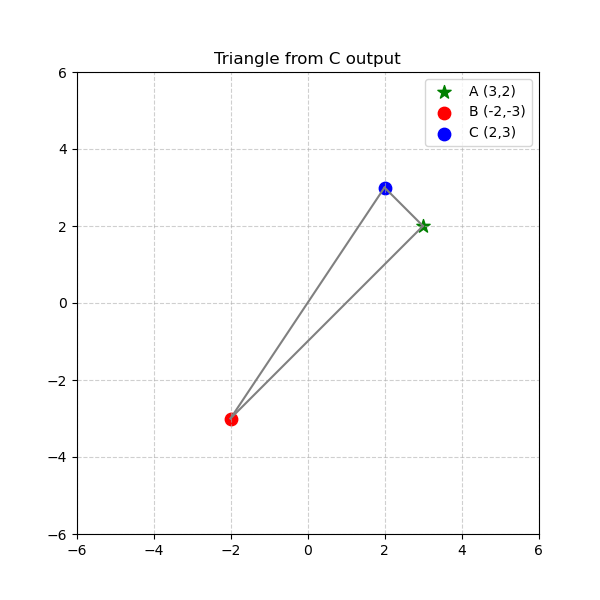
\includegraphics[width=\columnwidth, height=0.8\textheight, keepaspectratio]{fig3.1.png}     
\end{frame}

    \begin{frame}[fragile]
\frametitle{Python and C Code}

\begin{lstlisting}
import subprocess
import matplotlib.pyplot as plt

# Compile the C code
subprocess.run(["gcc", "triangle.c", "-o", "triangle"])

# Run the compiled program and capture output
result = subprocess.run(["./triangle"], capture_output=True, text=True)
coords = list(map(int, result.stdout.split()))

# Extract points
A = (coords[0], coords[1])
B = (coords[2], coords[3])
C = (coords[4], coords[5])


\end{lstlisting}

\end{frame}


  \begin{frame}[fragile]
\frametitle{Python and C Code}

\begin{lstlisting}
# ---- Plot in Python ----
fig, ax = plt.subplots(figsize=(6,6))
ax.plot([A[0],B[0]],[A[1],B[1]],'gray')
ax.plot([B[0],C[0]],[B[1],C[1]],'gray')
ax.plot([C[0],A[0]],[C[1],A[1]],'gray')

ax.scatter(*A,color='green',s=100,marker='*',label="A (3,2)")
ax.scatter(*B,color='red',s=80,label="B (-2,-3)")
ax.scatter(*C,color='blue',s=80,label="C (2,3)")
\end{lstlisting}

\end{frame}

    \begin{frame}[fragile]
\frametitle{Python and C Code}

\begin{lstlisting}
ax.set_aspect("equal","box")
ax.set_xlim(-6,6)
ax.set_ylim(-6,6)
ax.grid(True,linestyle="--",alpha=0.6)
ax.set_title("Triangle from C output")
ax.legend()
plt.savefig("fig3.1.png")
plt.show()
\end{lstlisting}

\end{frame}


\begin{frame}{Plot-Using  Python}
\textbf{Graph representation:}
\begin{figure}[H]
    \centering
 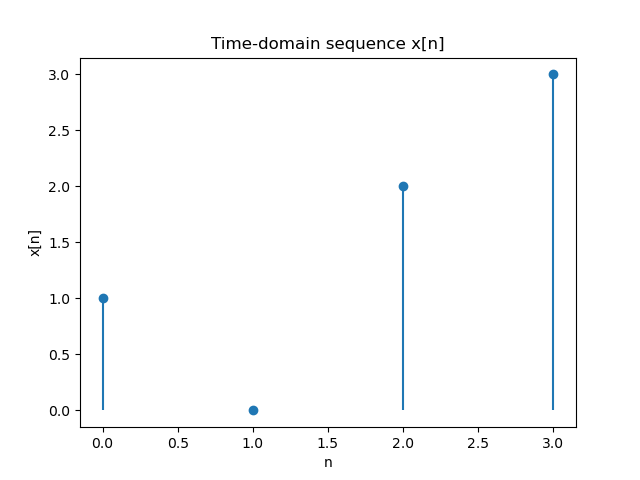
\includegraphics[width=0.5\linewidth]{fig3.png}
    \caption{0}
    \label{fig:placeholder}
\end{figure}
\end{frame}
\end{document}

